\documentclass[11pt,a4paper]{article}

\usepackage[T1]{fontenc}
\usepackage[utf8]{inputenc}
\usepackage{amsmath,amsthm}
\usepackage{newtxtext,newtxmath}
\usepackage[varqu]{zi4}
\usepackage{microtype}
\usepackage[margin=1in]{geometry}
\usepackage{array,booktabs,tabularx}
\usepackage[dvipsnames]{xcolor}
\usepackage{tikz}
\usetikzlibrary{positioning,arrows.meta,shapes.geometric,calc,fit,backgrounds,decorations.pathreplacing}
\usepackage{pgfplots}
\pgfplotsset{compat=1.18}
\usepackage{listings}
\usepackage[most]{tcolorbox}
\usepackage[font=small,labelfont=bf]{caption}
\usepackage{enumitem}
\usepackage[colorlinks,linkcolor=MidnightBlue,citecolor=MidnightBlue,urlcolor=MidnightBlue]{hyperref}
\usepackage[nameinlink]{cleveref}

% ---------------------------------------------------------------- notation
\newcommand{\ins}[1]{\textsf{#1}}
\newcommand{\clo}[2]{[#1 : #2]}
\newcommand{\pr}[2]{(#1,\, #2)}
\newcommand{\unit}{()}
\newcommand{\sem}[1]{[\![#1]\!]}
\newcommand{\trans}{\;\longrightarrow\;}
\newcommand{\cs}[3]{\langle #1,\ #2,\ #3\rangle}
\newcommand{\seq}{\mathbin{;}}
\newcommand{\cat}[1]{\mathrm{#1}}
\newcommand{\tpair}[2]{\langle #1, #2\rangle}

% term = blue, code = orange, stack = green, heap = purple
\definecolor{tfill}{HTML}{DCE9F7}
\definecolor{sfill}{HTML}{DDF0DC}
\definecolor{cfill}{HTML}{FCE8D2}
\definecolor{hfill}{HTML}{F1DDEE}
\definecolor{tline}{HTML}{2F6DB5}
\definecolor{sline}{HTML}{3C8A3A}
\definecolor{cline}{HTML}{C7701C}
\definecolor{hline}{HTML}{9A3F8E}

\tikzset{
  >=Stealth,
  every picture/.append style={font=\small},
  ptr/.style={->, thick},
  regbox/.style={draw=#1, thick, rounded corners=3pt, align=center, minimum width=2.6cm, minimum height=1.5cm},
  half/.style={draw, minimum width=0.75cm, minimum height=0.6cm, inner sep=1pt, fill=white},
  tag/.style={draw, minimum width=0.55cm, minimum height=0.6cm, inner sep=1pt, font=\scriptsize\sffamily},
  scell/.style={draw=sline, fill=sfill, minimum width=1.9cm, minimum height=0.5cm, font=\footnotesize, inner sep=1pt},
}

\theoremstyle{definition}
\newtheorem{definition}{Definition}
\newtheorem{exercise}{Exercise}
\theoremstyle{plain}
\newtheorem{theorem}{Theorem}

\newtcolorbox{aside}[1]{enhanced, breakable, colback=black!3, colframe=black!35,
  boxrule=0.5pt, arc=2pt, fonttitle=\bfseries\small, title={#1}, coltitle=black,
  colbacktitle=black!10, left=6pt, right=6pt}

\lstdefinelanguage{vm16}{morekeywords={LI,MOV,LW,SW,LB,SB,LWA,SWA,ADD,SUB,AND,OR,XOR,MUL,DIVU,
  NOT,NEG,SHL,SHR,SAR,ADDI,BEQ,BNE,BLT,BGE,BLTU,BGEU,BZ,BNZ,JMP,JR,PUSH,POP,GETDSP,SETDSP,
  CALL,CALLR,RET,SYS,HALT},
  sensitive=true, morecomment=[l]{;}}
\lstset{language=vm16, basicstyle=\ttfamily\small, keywordstyle=\bfseries,
  commentstyle=\color{black!55}, columns=fullflexible, keepspaces,
  frame=single, rulecolor=\color{black!30}, xleftmargin=6pt, xrightmargin=6pt,
  aboveskip=8pt, belowskip=8pt, tabsize=8}
\lstdefinestyle{cam}{language={}, keywordstyle={}, morecomment=[l]{\%}}

\title{The Categorical Abstract Machine\\[4pt]\large A Tutorial Introduction}
\author{}
\date{\today}

\begin{document}
\maketitle

\begin{abstract}
\noindent
The Categorical Abstract Machine (CAM) of Cousineau, Curien and Mauny is a
small and elegant machine for the call-by-value $\lambda$-calculus. It gave the
Caml language its name. Its origins lie in category theory, but the machine
itself needs none: it is what you get from the SECD machine if you replace
variable names by positions, represent environments as nested pairs, and
compile programs ahead of time. Three registers are then enough, and the
whole instruction set fits on half a page. This tutorial develops the machine
from those ideas, gives its transition rules and its compiler, and traces
several programs step by step, including a recursive factorial. It then
explains, without assuming any category theory, where the name comes from:
the compiled code is a composition of a handful of functions on pairs, and the
laws those functions obey are the laws of a cartesian closed category. A final
part looks at a complete implementation on the VM16 virtual machine, with a
copying garbage collector, and measures it against the SECD machine and against
hand-written code. The prerequisites are the untyped $\lambda$-calculus and,
ideally, the companion tutorial on the SECD machine.
\end{abstract}

\tableofcontents

% =====================================================================
\section{Introduction}

In 1964 Peter Landin showed how to evaluate $\lambda$-terms with a
machine~\cite{landin64}. His SECD machine keeps four lists: a stack S of
values, an environment E that maps names to values, a control C of
expressions still to be evaluated, and a dump D of suspended calls. Twenty
years later, Guy Cousineau, Pierre-Louis Curien and Michel Mauny proposed a
different machine~\cite{cam85,cam87}. It came out of Curien's work on
\emph{categorical combinators}~\cite{curien86}, a way of translating
$\lambda$-terms into a few combinators taken from category theory. Running
those combinators directly gave the \emph{Categorical Abstract Machine}.

The CAM turned out to be very practical. It was the target of the first
implementation of ML at INRIA, and the language took its name from it: Caml is
the \emph{Categorical Abstract Machine Language}. Later Caml systems moved to
other machines~\cite{leroy90}, but the CAM remains one of the clearest
examples of how to compile a functional language.

This tutorial approaches the CAM from the SECD side. We will see that three
design changes turn Landin's machine into the CAM:

\begin{enumerate}[itemsep=2pt]
\item \textbf{Positions instead of names.} A variable is replaced by its
  distance from its binder, its \emph{de Bruijn index}, so that the machine
  never searches for a name.
\item \textbf{Environments are values.} An environment is a chain of nested
  pairs, so it can sit in the same register as any other value. The SECD
  machine's S and E collapse into a single register, the \emph{term}.
\item \textbf{Compile first.} The program is translated once into a sequence
  of instructions, so there is no expression tree to take apart at run time.
  Return addresses go on the stack, and the dump disappears.
\end{enumerate}

\Cref{sec:fromsecd} develops these ideas, and \cref{sec:machine} gives the
machine. \Cref{sec:compiling} shows how to compile to it, and
\cref{sec:examples,sec:recursion} run programs, ending with a factorial.
\Cref{sec:categorical} explains the categorical reading, and
\cref{sec:vm16,sec:measure} present and measure a complete implementation. A
reference card, \cref{sec:card}, collects the rules on one page.

\begin{aside}{What you need to know}
We assume the untyped $\lambda$-calculus: terms $x$, $\lambda x.M$ and $M\,N$,
free and bound variables, and $\beta$-reduction. We use call-by-value: a
function's argument is evaluated before the call, and evaluation stops at a
$\lambda$. The companion tutorial \emph{The SECD Machine} covers environments
and closures in detail; we review them briefly here. No category theory is
needed anywhere.
\end{aside}

The examples use the input language of the implementation in
\cref{sec:vm16}: single-letter variables, $\verb|\x y.M|$ for
$\lambda x.\lambda y.M$, integers, the curried operators
\verb|+ - * / % = <|, a conditional \verb|if c t e|, and recursive functions
\verb|rec f.\x.M|.

% =====================================================================
\section{From the SECD machine to the CAM}\label{sec:fromsecd}

\subsection{Environments and closures, briefly}

An abstract machine for the $\lambda$-calculus avoids substitution. Instead of
replacing $x$ by a value in the body of $\lambda x.M$, it evaluates $M$ in an
\emph{environment} that records the value of $x$. A function value must then
remember the environment it was created in, so that its free variables keep
the meaning they had there. The pair of code and environment is a
\emph{closure}. Both ideas carry over unchanged to the CAM; what changes is
how environments are represented.

\subsection{From names to positions}

In the SECD machine, the environment is a list of bindings
$[x\mapsto 4,\ y\mapsto 3,\ \dots]$, and every variable occurrence is looked
up by comparing names. That is wasted work: the shape of the environment at
any point of a program is known before the program runs. In
$\lambda a.\lambda b.a$, the body $a$ always runs in an environment whose
newest binding is $b$ and whose next binding is $a$. So $a$ can be compiled to
``the second binding'', and the name can be thrown away.

\begin{definition}
The \emph{de Bruijn index} of a variable occurrence is the number of
$\lambda$s between the occurrence and its binder~\cite{debruijn72}. Index 0
refers to the innermost enclosing $\lambda$.
\end{definition}

\Cref{fig:debruijn} shows the indices for a small term. The same variable can
have different indices at different occurrences, because the count depends
on where the occurrence is.

\begin{figure}[t]
\centering
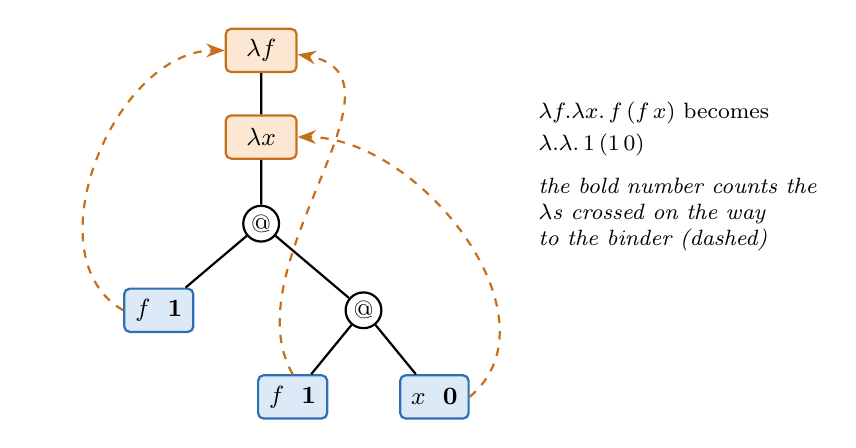
\begin{tikzpicture}[
  lam/.style={draw=cline, fill=cfill, thick, rounded corners=2pt, minimum width=0.9cm, minimum height=0.55cm},
  app/.style={draw, thick, circle, inner sep=1.2pt, fill=white},
  var/.style={draw=tline, fill=tfill, thick, rounded corners=2pt, minimum height=0.55cm, inner xsep=4pt},
  level distance=1.05cm]
\node[lam] (f) at (0,0) {$\lambda f$};
\node[lam] (x) at (0,-1.1) {$\lambda x$};
\node[app] (a1) at (0,-2.2) {$@$};
\node[var] (f1) at (-1.3,-3.3) {$f$ \ \textbf{1}};
\node[app] (a2) at (1.3,-3.3) {$@$};
\node[var] (f2) at (0.4,-4.4) {$f$ \ \textbf{1}};
\node[var] (x1) at (2.2,-4.4) {$x$ \ \textbf{0}};
\draw[thick] (f) -- (x) -- (a1) -- (f1);
\draw[thick] (a1) -- (a2) -- (f2);
\draw[thick] (a2) -- (x1);
\draw[->, dashed, cline, thick] (f1.west) to[out=150, in=180] (f.west);
\draw[->, dashed, cline, thick] (x1.east) to[out=40, in=0] (x.east);
\draw[->, dashed, cline, thick] (f2.north) to[out=120, in=-10] ($(f.east)+(0,-0.05)$);
\node[align=left, font=\footnotesize, anchor=west] at (3.4,-1.6)
  {$\lambda f.\lambda x.\,f\,(f\,x)$ becomes\\[2pt] $\lambda.\lambda.\,1\,(1\,0)$\\[6pt]
   \textit{the bold number counts the}\\ \textit{$\lambda$s crossed on the way}\\ \textit{to the binder (dashed)}};
\end{tikzpicture}
\caption{De Bruijn indices for the Church numeral 2. Each variable is
replaced by the number of $\lambda$s between it and its binder.}
\label{fig:debruijn}
\end{figure}

\subsection{Environments as nested pairs}

If variables are positions, an environment no longer needs names; it only
needs to hold values in order. The CAM uses the simplest structure that does
this, a chain of pairs. The empty environment is the empty tuple $\unit$, and
binding a new value $v$ in environment $e$ gives the pair $\pr{e}{v}$. Inside
$\lambda a.\lambda b.\dots$, applied to 4 and 3, the environment is
\[
  \pr{\pr{\unit}{4}}{3}.
\]
The newest value is always the second component of the outermost pair, the
next one is one step further in, and so on. The variable with index $i$ is
found by taking the first component $i$ times and then the second component
once (\cref{fig:pairs}):
\[
  \text{index } i \quad\longmapsto\quad
  \underbrace{\mathit{fst}\seq\cdots\seq\mathit{fst}}_{i}\seq\mathit{snd}.
\]

\begin{figure}[t]
\centering
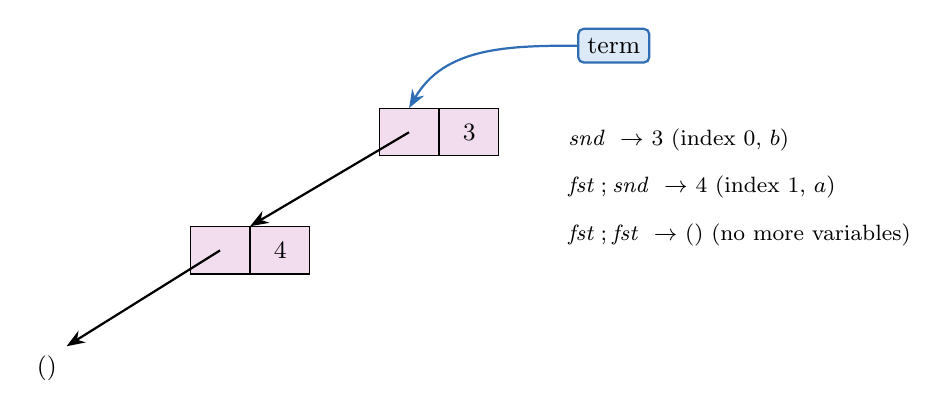
\begin{tikzpicture}
\node[half, fill=hfill] (p1a) at (0,0) {};
\node[half, fill=hfill, right=0pt of p1a] (p1b) {$3$};
\node[half, fill=hfill] (p2a) at (-2.4,-1.5) {};
\node[half, fill=hfill, right=0pt of p2a] (p2b) {$4$};
\node[font=\small] (u) at (-4.6,-3.0) {$\unit$};
\draw[ptr] (p1a.center) -- (p2a.north east);
\draw[ptr] (p2a.center) -- (u.north east);
\node[draw=tline, fill=tfill, thick, rounded corners=2pt] (t) at (2.6,1.1) {term};
\draw[ptr, tline] (t.west) to[out=180, in=60] (p1a.north);
\node[anchor=west, font=\footnotesize, align=left] at (1.9,-0.1) {$\mathit{snd}$ \;$\to$ 3 \hfill (index 0, $b$)};
\node[anchor=west, font=\footnotesize, align=left] at (1.9,-0.7) {$\mathit{fst}\seq\mathit{snd}$ \;$\to$ 4 \hfill (index 1, $a$)};
\node[anchor=west, font=\footnotesize, align=left] at (1.9,-1.3) {$\mathit{fst}\seq\mathit{fst}$ \;$\to$ $\unit$ \hfill (no more variables)};
\end{tikzpicture}
\caption{The environment $\pr{\pr{\unit}{4}}{3}$ as heap cells. Each pair
has a first field (left half) pointing to the older environment and a
second field (right half) holding a value. Variables are reached by following first fields.}
\label{fig:pairs}
\end{figure}

Two things follow. First, extending an environment is a single allocation, and
the old environment is shared, not copied. Second, an environment is an
ordinary value. Pairs are values in the CAM, so a single register can hold
either an environment or the result of a computation, and the instructions
that save and restore one also work for the other.

\subsection{One register for S and E}

The SECD machine keeps the current environment in E and intermediate values
on S. The CAM merges the two into one register, the \emph{term}. At the start
of evaluating an expression the term holds the environment, and at the end it
holds the expression's value. In between, environments that will be needed
again are saved on the stack.

The dump goes as well. Because the CAM runs compiled code, a pending call only
needs to remember where to continue, a single code address, and that address
fits on the same stack. \Cref{fig:registers} compares the two machines.

\begin{figure}[t]
\centering
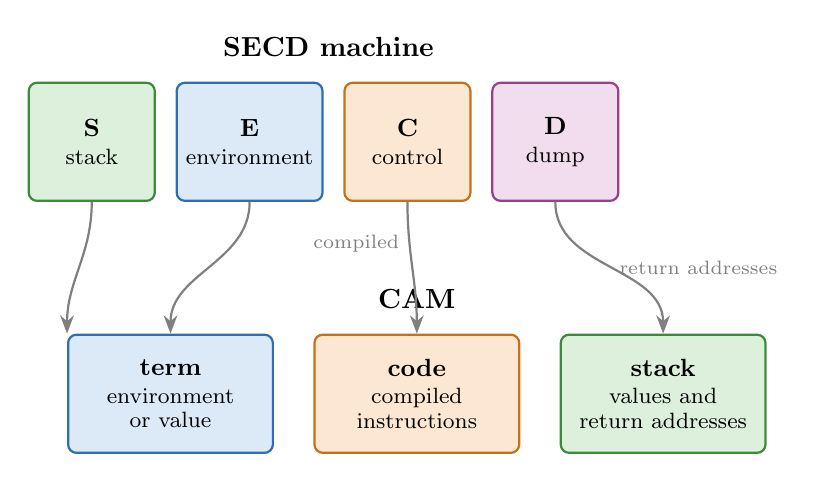
\begin{tikzpicture}
\node[regbox=sline, fill=sfill, minimum width=1.6cm] (S) at (0,0) {\textbf{S}\\[-1pt]\footnotesize stack};
\node[regbox=tline, fill=tfill, minimum width=1.6cm, right=0.25cm of S] (E) {\textbf{E}\\[-1pt]\footnotesize environment};
\node[regbox=cline, fill=cfill, minimum width=1.6cm, right=0.25cm of E] (C) {\textbf{C}\\[-1pt]\footnotesize control};
\node[regbox=hline, fill=hfill, minimum width=1.6cm, right=0.25cm of C] (D) {\textbf{D}\\[-1pt]\footnotesize dump};
\node[font=\bfseries, above=0.2cm of $(E.north)!0.5!(C.north)$] {SECD machine};
\node[regbox=tline, fill=tfill] (T) at (1.0,-3.2) {\textbf{term}\\[-1pt]\footnotesize environment\\[-2pt]\footnotesize or value};
\node[regbox=cline, fill=cfill, right=0.5cm of T] (K) {\textbf{code}\\[-1pt]\footnotesize compiled\\[-2pt]\footnotesize instructions};
\node[regbox=sline, fill=sfill, right=0.5cm of K] (St) {\textbf{stack}\\[-1pt]\footnotesize values and\\[-2pt]\footnotesize return addresses};
\node[font=\bfseries, above=0.2cm of K.north] {CAM};
\draw[->, thick, black!50] (S.south) to[out=-90, in=90] (T.north west);
\draw[->, thick, black!50] (E.south) to[out=-90, in=90] (T.north);
\draw[->, thick, black!50] (C.south) to[out=-90, in=90] node[pos=0.3, left, font=\scriptsize] {compiled} (K.north);
\draw[->, thick, black!50] (D.south) to[out=-90, in=90] node[pos=0.5, right, font=\scriptsize] {return addresses} (St.north);
\end{tikzpicture}
\caption{The SECD machine's four registers and the CAM's three. The term
takes over the roles of S and E, compiled code replaces the control, and
return addresses on the stack replace the dump. The stack also keeps the
intermediate values that S used to hold.}
\label{fig:registers}
\end{figure}

% =====================================================================
\section{The machine}\label{sec:machine}

\subsection{Values and states}

The CAM manipulates four kinds of value:
\begin{itemize}[itemsep=1pt]
\item numbers $n$;
\item the empty tuple $\unit$, the empty environment;
\item pairs $\pr{s}{t}$ of values;
\item closures $\clo{C}{s}$, a piece of code $C$ together with the
  environment $s$ it was created in.
\end{itemize}
A state is a triple $\cs{t}{C}{S}$: the term $t$, the code $C$ still to run,
and the stack $S$. We write $c\seq C$ for code starting with instruction $c$,
and $v.S$ for a stack with $v$ on top. The stack holds values and also code
sequences, which act as return addresses. A program $P$ starts in the state
$\cs{\unit}{P}{\varepsilon}$, with the empty environment and an empty stack,
and stops when it reaches the instruction \ins{STOP}; the term is then the
result.

\subsection{Instructions}

\Cref{fig:rules} gives the whole machine. There are four groups.

\begin{figure}[t]
\centering
\small
\renewcommand{\arraystretch}{1.25}
\begin{tabular}{@{}l r@{\;}c@{\;}l@{}}
\toprule
& \multicolumn{3}{c}{$\cs{\text{term}}{\text{code}}{\text{stack}} \trans \cs{\text{term}}{\text{code}}{\text{stack}}$}\\
\midrule
\ins{ACC} $i$ & $\cs{t}{\ins{ACC}\,i\seq C}{S}$ &$\trans$& $\cs{\mathit{snd}(\mathit{fst}^i(t))}{C}{S}$\\
\ins{QUOTE} $n$ & $\cs{t}{\ins{QUOTE}\,n\seq C}{S}$ &$\trans$& $\cs{n}{C}{S}$\\
\midrule
\ins{PUSH} & $\cs{t}{\ins{PUSH}\seq C}{S}$ &$\trans$& $\cs{t}{C}{t.S}$\\
\ins{SWAP} & $\cs{t}{\ins{SWAP}\seq C}{s.S}$ &$\trans$& $\cs{s}{C}{t.S}$\\
\ins{CONS} & $\cs{t}{\ins{CONS}\seq C}{s.S}$ &$\trans$& $\cs{\pr{s}{t}}{C}{S}$\\
\midrule
\ins{CUR} $C'$ & $\cs{t}{\ins{CUR}\,C'\seq C}{S}$ &$\trans$& $\cs{\clo{C'}{t}}{C}{S}$\\
\ins{APP} & $\cs{\pr{\clo{C'}{s}}{t}}{\ins{APP}\seq C}{S}$ &$\trans$& $\cs{\pr{s}{t}}{C'}{C.S}$\\
\ins{RET} & $\cs{t}{\ins{RET}\seq C}{C'.S}$ &$\trans$& $\cs{t}{C'}{S}$\\
\midrule
\ins{op} & $\cs{n_2}{\textit{op}\seq C}{n_1.S}$ &$\trans$& $\cs{n_1 \mathbin{\textit{op}} n_2}{C}{S}$\\
\ins{BRANCH} $C_1\,C_2$ & $\cs{b}{\ins{BRANCH}\,C_1\,C_2\seq C}{s.S}$ &$\trans$& $\cs{s}{C_b\seq C}{S}$
  \quad $C_b = C_1$ if $b\neq 0$, else $C_2$\\
\ins{REC} $C'$ & $\cs{t}{\ins{REC}\,C'\seq C}{S}$ &$\trans$& $\cs{k}{C}{S}$ \quad where $k = \clo{C'}{\pr{t}{k}}$\\
\bottomrule
\end{tabular}
\caption{The transition rules of the CAM. \ins{ACC}, \ins{QUOTE} load the
term; \ins{PUSH}, \ins{SWAP}, \ins{CONS} manage the stack; \ins{CUR},
\ins{APP}, \ins{RET} create and call functions; the last group adds
arithmetic, conditionals and recursion.}
\label{fig:rules}
\end{figure}

\begin{description}[style=nextline, leftmargin=1.2em, itemsep=3pt]
\item[Loading the term.] $\ins{ACC}\,i$ replaces the environment in the term
  by the value of variable $i$. The original CAM has separate instructions
  \ins{FST} and \ins{SND}; \ins{ACC}~$i$ abbreviates $i$ \ins{FST}s and one
  \ins{SND}. $\ins{QUOTE}\,n$ replaces the term by a constant.
\item[The stack.] \ins{PUSH} saves a copy of the term. \ins{SWAP} exchanges
  the term with the top of the stack: typically it saves a result and brings
  back a saved environment. \ins{CONS} pairs the top of the stack with the
  term. These three are all the CAM needs to evaluate two expressions in the
  same environment and combine their values (\cref{sec:dance}).
\item[Functions.] $\ins{CUR}\,C'$ makes a closure of the code $C'$ and the
  current environment; its name comes from \emph{currying}. \ins{APP} expects a
  pair of a closure $\clo{C'}{s}$ and an argument $t$. It builds the closure's
  environment extended with the argument, $\pr{s}{t}$, pushes the rest of the
  code as a return address, and jumps to $C'$. When $C'$ finishes, \ins{RET}
  pops the return address.
\item[Extensions.] Arithmetic operators take their left operand from the
  stack and their right operand from the term. \ins{BRANCH} tests the term,
  restores a saved environment, and continues with one of two code sequences.
  \ins{REC} builds a closure that contains itself, for recursive functions.
  None of these is part of the categorical core; \cref{sec:recursion}
  discusses them.
\end{description}

Notice how little each instruction does. There is no rule that walks a list
of bindings, no rule that takes an expression tree apart, and no rule that
saves three registers at once. Every transition does a constant amount of work
except \ins{ACC}~$i$, which takes $i+1$ steps, and only \ins{CUR}, \ins{CONS},
\ins{APP} and \ins{REC} allocate memory.

% =====================================================================
\section{Compiling for the CAM}\label{sec:compiling}

\subsection{The compiler}

The compiler translates a term $M$ into code $\sem{M}_\rho$, where $\rho$ is
the list of variable names in scope, innermost first. The position of a name
in $\rho$ is its de Bruijn index:
\begin{align*}
\sem{x}_\rho &= \ins{ACC}\ i \qquad\text{where $x$ is at position $i$ in $\rho$}\\
\sem{n}_\rho &= \ins{QUOTE}\ n\\
\sem{\lambda x.M}_\rho &= \ins{CUR}\ (\sem{M}_{x:\rho}\seq \ins{RET})\\
\sem{M\,N}_\rho &= \ins{PUSH}\seq \sem{M}_\rho\seq \ins{SWAP}\seq \sem{N}_\rho\seq \ins{CONS}\seq \ins{APP}
\end{align*}
That is the whole compiler for the pure $\lambda$-calculus. The extensions add
\begin{align*}
\sem{\textit{op}\ M\ N}_\rho &= \ins{PUSH}\seq \sem{M}_\rho\seq \ins{SWAP}\seq \sem{N}_\rho\seq \textit{op}\\
\sem{\textbf{if}\ c\ t\ e}_\rho &= \ins{PUSH}\seq \sem{c}_\rho\seq \ins{BRANCH}\ \sem{t}_\rho\ \sem{e}_\rho\\
\sem{\textbf{rec}\ f.\lambda x.M}_\rho &= \ins{REC}\ (\sem{M}_{x:f:\rho}\seq \ins{RET})
\end{align*}
and an operator used on its own, such as \verb|(+ 1)|, is first expanded to
$\lambda a.\lambda b.\,\textit{op}\ a\ b$.

The compiler has one invariant that makes everything fit together:

\begin{theorem}[Code leaves the stack as it found it]\label{thm:invariant}
If $M$ evaluates to the value $v$ in environment $e$, then
\[
  \cs{e}{\sem{M}_\rho\seq C}{S} \trans^{*} \cs{v}{C}{S},
\]
where $\rho$ lists the names whose values $e$ holds.
\end{theorem}

\begin{proof}[Proof sketch]
By induction on $M$. For a variable, \ins{ACC}~$i$ walks $e$ to the value. For
$\lambda x.M$, \ins{CUR} turns $e$ into the closure, which is a value. For
$M\,N$ we follow the code. \ins{PUSH} saves $e$. By induction $\sem{M}$ turns
$e$ into a closure $\clo{C'}{s}$ without disturbing the stack, so \ins{SWAP}
leaves $e$ in the term and the closure on the stack. By induction again
$\sem{N}$ turns $e$ into the argument $a$, \ins{CONS} builds
$\pr{\clo{C'}{s}}{a}$, and \ins{APP} runs $C'$ on $\pr{s}{a}$ with $C$ pushed.
$C'$ is $\sem{B}_{y:\rho'}\seq\ins{RET}$ for the function's body $B$, so by
induction it ends with the result in the term and $C$ on top of the stack,
and \ins{RET} continues with $C$ and $S$.
\end{proof}

\subsection{The pairing dance}\label{sec:dance}

The heart of the compiler is the application rule. To evaluate $M\,N$, both
$M$ and $N$ must be evaluated \emph{in the same environment}, but evaluating
$M$ replaces the environment in the term by $M$'s value. \ins{PUSH},
\ins{SWAP} and \ins{CONS} solve this by parking values on the stack, as
\cref{fig:dance} shows. The same pattern appears every time two values have
to be computed from one environment: for applications, for operators, and in
the categorical reading of \cref{sec:categorical}, for pairing in general.

\begin{figure}[t]
\centering
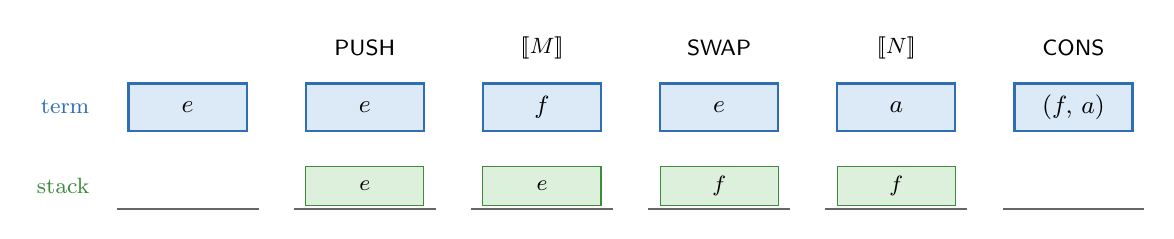
\begin{tikzpicture}[x=2.25cm]
\foreach \i/\ins/\t/\s in {
  0/{}/{$e$}/{},
  1/PUSH/{$e$}/{$e$},
  2/{$\sem{M}$}/{$f$}/{$e$},
  3/SWAP/{$e$}/{$f$},
  4/{$\sem{N}$}/{$a$}/{$f$},
  5/CONS/{$\pr{f}{a}$}/{}} {
  \node[draw=tline, fill=tfill, thick, minimum width=1.5cm, minimum height=0.6cm] at (\i, 0) {\t};
  \ifx\s\empty\else\node[scell, minimum width=1.5cm] at (\i, -1.0) {\s};\fi
  \draw[thick, black!60] (\i-0.4, -1.3) -- (\i+0.4, -1.3);
  \node[font=\footnotesize\sffamily] at (\i, 0.75) {\ins};
}
\node[anchor=east, font=\footnotesize, tline] at (-0.5,0) {term};
\node[anchor=east, font=\footnotesize, sline] at (-0.5,-1.0) {stack};
\end{tikzpicture}
\caption{Evaluating $M$ and $N$ in the same environment $e$. \ins{PUSH}
saves $e$; $\sem{M}$ computes the function $f$; \ins{SWAP} parks $f$ and
restores $e$; $\sem{N}$ computes the argument $a$; \ins{CONS} pairs them. The
stack below the line is the same before and after.}
\label{fig:dance}
\end{figure}

\subsection{An example}

Compiling $(\lambda x.\,{+}\;x\;1)\;41$ in the empty environment gives
\begin{lstlisting}[style=cam]
PUSH
CUR  (PUSH; ACC 0; SWAP; QUOTE 1; ADD; RET)    % \x. + x 1
SWAP
QUOTE 41
CONS
APP
STOP
\end{lstlisting}
The outer \ins{PUSH}\dots\ins{APP} is the application rule, with
$\sem{\lambda x.\,{+}\;x\;1}$ and $\sem{41}$ in the two slots. Inside the
closure, the operator rule computes $x+1$, where $x$ is \ins{ACC}~0 because
it is the innermost (and only) variable. \ins{STOP} is added after the whole
program.

In memory, code is a flat sequence of bytes, so the nested code of a \ins{CUR}
is laid out inline, preceded by the address where the code continues. The
implementation's disassembler prints the example as
\begin{lstlisting}[style=cam]
3000  PUSH
3001  CUR 300D          % the closure's code is 3004..300C
3004    PUSH
3005    ACC 0
3007    SWAP
3008    QUOTE 1
300B    ADD
300C    RET
300D  SWAP
300E  QUOTE 41
3011  CONS
3012  APP
3013  STOP
\end{lstlisting}
Thirteen instructions, seven of them at the top level. The next section runs
it.

% =====================================================================
\section{Worked examples}\label{sec:examples}

The traces in this section were produced by replaying the code that the
implementation of \cref{sec:vm16} compiled, and they agree with it step for
step. Each row shows the state \emph{before} the instruction in the last
column is executed. Return addresses are written $r$, and closures are written
with the label of their code.

\subsection{A function call}

\Cref{tab:trace1} traces $(\lambda x.\,{+}\;x\;1)\;41$; let $B$ be the code
of the closure. Rows 0--5 build the pair of function and argument. Row 5
calls it: \ins{APP} replaces $\pr{\clo{B}{\unit}}{41}$ by the environment
$\pr{\unit}{41}$, pushes the return address, and jumps to $B$. In the body,
rows 6--10 are the operator rule, with $x$ fetched by \ins{ACC}~0, and
\ins{RET} goes back to \ins{STOP}.

\begin{table}[t]
\centering
\small
\begin{tabular}{@{}r l l l@{}}
\toprule
& term & stack & next\\
\midrule
0 & $\unit$ & $\varepsilon$ & \ins{PUSH}\\
1 & $\unit$ & $\unit$ & \ins{CUR} $B$\\
2 & $\clo{B}{\unit}$ & $\unit$ & \ins{SWAP}\\
3 & $\unit$ & $\clo{B}{\unit}$ & \ins{QUOTE} 41\\
4 & $41$ & $\clo{B}{\unit}$ & \ins{CONS}\\
5 & $\pr{\clo{B}{\unit}}{41}$ & $\varepsilon$ & \ins{APP}\\
6 & $\pr{\unit}{41}$ & $r$ & \ins{PUSH}\\
7 & $\pr{\unit}{41}$ & $\pr{\unit}{41}.\,r$ & \ins{ACC} 0\\
8 & $41$ & $\pr{\unit}{41}.\,r$ & \ins{SWAP}\\
9 & $\pr{\unit}{41}$ & $41.\,r$ & \ins{QUOTE} 1\\
10 & $1$ & $41.\,r$ & \ins{ADD}\\
11 & $42$ & $r$ & \ins{RET}\\
12 & $42$ & $\varepsilon$ & \ins{STOP}\\
\bottomrule
\end{tabular}
\caption{The CAM evaluating $(\lambda x.\,{+}\;x\;1)\;41$. $B$ is the code
\ins{PUSH; ACC 0; SWAP; QUOTE 1; ADD; RET}, and $r$ the return address of
\ins{STOP}.}
\label{tab:trace1}
\end{table}

Compare this with the SECD machine. There, the same call creates a dump frame
holding three registers, and the body runs with a fresh stack. Here the call
pushes one word, and the body uses the caller's stack, above the return
address.

\subsection{Two arguments: \texorpdfstring{$K\,4\,3$}{K 4 3}}

The combinator $K = \lambda a.\lambda b.a$ shows how curried functions and
closures interact. Its body $a$ has index 1, so $\sem{K} = \ins{CUR}\,K_1$
with
\[
  K_1 = \ins{CUR}\ K_2\seq \ins{RET}, \qquad K_2 = \ins{ACC}\ 1\seq \ins{RET}.
\]
\Cref{tab:trace2} traces $K\,4\,3$, which is $(K\,4)\,3$. The first \ins{APP}
(row 6) calls $K_1$ with the environment $\pr{\unit}{4}$. $K_1$ does no more
than wrap that environment into a new closure $\clo{K_2}{\pr{\unit}{4}}$ and
return it (rows 7--8): this closure \emph{is} the partial application
$K\,4$, and the 4 is stored in its environment. The second \ins{APP} (row 12)
extends that environment with 3, so $K_2$ runs in $\pr{\pr{\unit}{4}}{3}$,
exactly the environment of \cref{fig:pairs}, and \ins{ACC}~1 finds the 4.

\begin{table}[t]
\centering
\small
\begin{tabular}{@{}r l l l@{}}
\toprule
& term & stack & next\\
\midrule
0 & $\unit$ & $\varepsilon$ & \ins{PUSH}\\
1 & $\unit$ & $\unit$ & \ins{PUSH}\\
2 & $\unit$ & $\unit.\unit$ & \ins{CUR} $K_1$\\
3 & $\clo{K_1}{\unit}$ & $\unit.\unit$ & \ins{SWAP}\\
4 & $\unit$ & $\clo{K_1}{\unit}.\unit$ & \ins{QUOTE} 4\\
5 & $4$ & $\clo{K_1}{\unit}.\unit$ & \ins{CONS}\\
6 & $\pr{\clo{K_1}{\unit}}{4}$ & $\unit$ & \ins{APP}\\
7 & $\pr{\unit}{4}$ & $r_1.\unit$ & \ins{CUR} $K_2$\\
8 & $\clo{K_2}{\pr{\unit}{4}}$ & $r_1.\unit$ & \ins{RET}\\
9 & $\clo{K_2}{\pr{\unit}{4}}$ & $\unit$ & \ins{SWAP}\\
10 & $\unit$ & $\clo{K_2}{\pr{\unit}{4}}$ & \ins{QUOTE} 3\\
11 & $3$ & $\clo{K_2}{\pr{\unit}{4}}$ & \ins{CONS}\\
12 & $\pr{\clo{K_2}{\pr{\unit}{4}}}{3}$ & $\varepsilon$ & \ins{APP}\\
13 & $\pr{\pr{\unit}{4}}{3}$ & $r_2$ & \ins{ACC} 1\\
14 & $4$ & $r_2$ & \ins{RET}\\
15 & $4$ & $\varepsilon$ & \ins{STOP}\\
\bottomrule
\end{tabular}
\caption{The CAM evaluating $K\,4\,3$. The closure created at row 8 is the
partial application $K\,4$.}
\label{tab:trace2}
\end{table}

\Cref{fig:app} shows the heap around the second call. The new environment
$\pr{s}{3}$ points to the closure's environment $s$ instead of copying it, so
any number of partial applications can share it.

\begin{figure}[t]
\centering
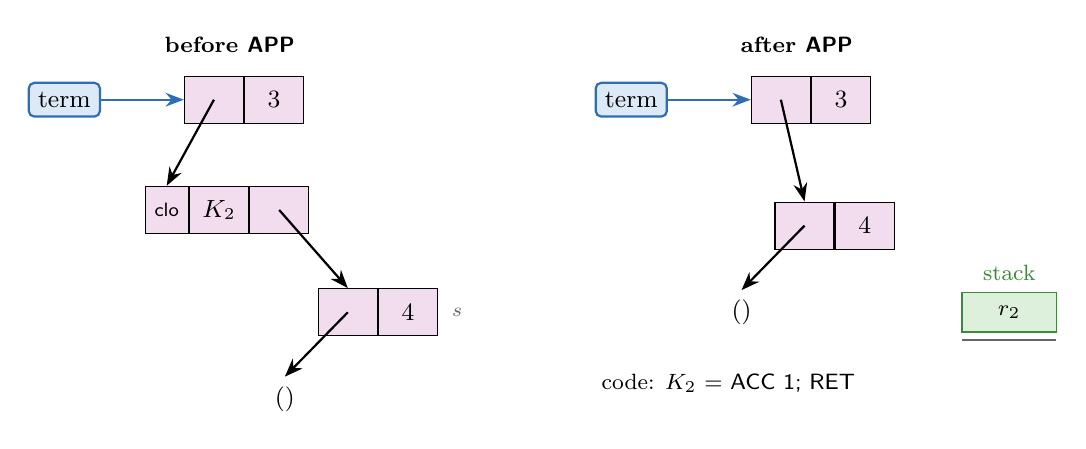
\begin{tikzpicture}
% before
\node[font=\bfseries\footnotesize] at (0.2,1.3) {before \ins{APP}};
\node[draw=tline, fill=tfill, thick, rounded corners=2pt] (t1) at (-1.9,0.6) {term};
\node[half, fill=hfill] (a) at (0,0.6) {};
\node[half, fill=hfill, right=0pt of a] (b) {$3$};
\node[tag, fill=hfill] (c1) at (-0.6,-0.8) {clo};
\node[half, fill=hfill, right=0pt of c1] (c2) {$K_2$};
\node[half, fill=hfill, right=0pt of c2] (c3) {};
\node[half, fill=hfill] (e1) at (1.7,-2.1) {};
\node[half, fill=hfill, right=0pt of e1] (e2) {$4$};
\node (u) at (0.9,-3.2) {$\unit$};
\draw[ptr, tline] (t1) -- (a.west);
\draw[ptr] (a.center) -- (c1.north);
\draw[ptr] (c3.center) -- (e1.north);
\draw[ptr] (e1.center) -- (u.north);
\node[font=\scriptsize, black!60, anchor=west] at ($(e2.east)+(0.05,0)$) {$s$};
% after
\begin{scope}[xshift=7.2cm]
\node[font=\bfseries\footnotesize] at (0.2,1.3) {after \ins{APP}};
\node[draw=tline, fill=tfill, thick, rounded corners=2pt] (t2) at (-1.9,0.6) {term};
\node[half, fill=hfill] (n1) at (0,0.6) {};
\node[half, fill=hfill, right=0pt of n1] (n2) {$3$};
\node[half, fill=hfill] (f1) at (0.3,-1.0) {};
\node[half, fill=hfill, right=0pt of f1] (f2) {$4$};
\node (u2) at (-0.5,-2.1) {$\unit$};
\draw[ptr, tline] (t2) -- (n1.west);
\draw[ptr] (n1.center) -- (f1.north);
\draw[ptr] (f1.center) -- (u2.north);
\node[scell, minimum width=1.2cm] (r) at (2.9,-2.1) {$r_2$};
\draw[thick, black!60] (2.3,-2.45) -- (3.5,-2.45);
\node[font=\footnotesize, sline] at (2.9,-1.6) {stack};
\node[font=\footnotesize, align=left, anchor=west] at (-2.4,-3.0) {code: $K_2$ = \ins{ACC 1; RET}};
\end{scope}
\end{tikzpicture}
\caption{The second call in $K\,4\,3$. Before: the term is the pair of the
closure $\clo{K_2}{s}$ and the argument 3. After: the term is $\pr{s}{3}$,
which shares $s$ with the closure, the return address is on the stack, and
the code is the closure's.}
\label{fig:app}
\end{figure}

% =====================================================================
\section{Conditionals and recursion}\label{sec:recursion}

\subsection{A conditional that evaluates one branch}

With call-by-value, a conditional cannot be an ordinary function: in
$\mathit{if}\ c\ t\ e$, both $t$ and $e$ would be evaluated before the call.
For Church booleans that is fatal in recursive definitions, because the
recursive branch is evaluated even when the base case applies. The SECD
tutorial works around this by wrapping both branches in a $\lambda d.$, and
Landin did the same in 1964. The CAM has the same problem with Church
booleans, since it is a call-by-value machine too: a factorial written with
Church booleans and without the wrappers recurses until memory runs out.

The cure is to make the conditional part of the compiler. The rule
\[
  \sem{\textbf{if}\ c\ t\ e}_\rho = \ins{PUSH}\seq \sem{c}_\rho\seq \ins{BRANCH}\ \sem{t}_\rho\ \sem{e}_\rho
\]
saves the environment, evaluates the condition, and then \ins{BRANCH} restores
the environment and runs only one of the two code sequences. In memory,
\ins{BRANCH} carries the address of the else-code, and the then-code ends
with a \ins{JUMP} past it:
\[
  \ins{PUSH}\seq \sem{c}\seq \ins{BRANCH}\ \mathit{else}\seq \sem{t}\seq
  \ins{JUMP}\ \mathit{end}\seq\ \mathit{else}{:}\ \sem{e}\seq\ \mathit{end}{:}
\]
This is the CAM's counterpart of the \ins{SEL} and \ins{JOIN} instructions of
the compiled SECD machine~\cite{henderson80}, but it needs no join: when the
chosen branch finishes, the machine simply continues with the next
instruction.

\subsection{Recursion}

The categorical combinators have no recursion. A recursive function can be
written with a fixpoint combinator; the call-by-value one is
\[
  Z = \lambda f.\,(\lambda x.\,f\,(\lambda y.\,x\,x\,y))\,(\lambda x.\,f\,(\lambda y.\,x\,x\,y)),
\]
and it works on the CAM unchanged. But it is slow: each recursive call goes
through two extra closures. Real implementations, including Caml's
\texttt{let rec}, build a closure that refers to itself instead:
\[
  \cs{t}{\ins{REC}\,C'\seq C}{S} \trans \cs{k}{C}{S}
  \qquad\text{where } k = \clo{C'}{\pr{t}{k}}.
\]
The closure's environment is the current one, extended with the closure
itself. When $k$ is called with argument $a$, its code runs in
$\pr{\pr{t}{k}}{a}$: the argument has index 0 and the function, under the name
$f$, has index 1. The cycle is created by allocating both cells and then
filling in their fields (\cref{fig:rec}).

\begin{figure}[t]
\centering
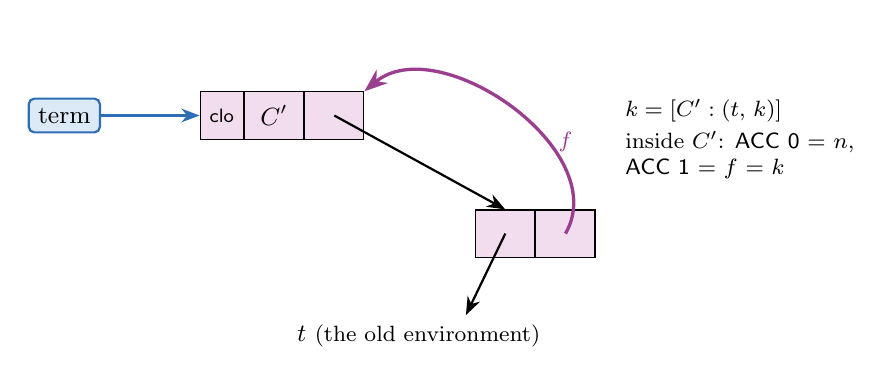
\begin{tikzpicture}
\node[draw=tline, fill=tfill, thick, rounded corners=2pt] (t) at (-3.0,0) {term};
\node[tag, fill=hfill] (k1) at (-1.0,0) {clo};
\node[half, fill=hfill, right=0pt of k1] (k2) {$C'$};
\node[half, fill=hfill, right=0pt of k2] (k3) {};
\node[half, fill=hfill] (p1) at (2.6,-1.5) {};
\node[half, fill=hfill, right=0pt of p1] (p2) {};
\node (e) at (1.5,-2.8) {$t$ \footnotesize(the old environment)};
\draw[ptr, tline] (t) -- (k1.west);
\draw[ptr] (k3.center) -- (p1.north);
\draw[ptr] (p1.center) -- ($(e.north)+(0.6,0)$);
\draw[ptr, hline, very thick] (p2.center) to[out=60, in=40] node[pos=0.35, right, font=\footnotesize] {$f$} (k3.north east);
\node[font=\footnotesize, anchor=west, align=left] at (4.0,-0.3) {$k = \clo{C'}{\pr{t}{k}}$\\[2pt] inside $C'$: \ins{ACC 0} = $n$,\\ \ins{ACC 1} = $f$ = $k$};
\end{tikzpicture}
\caption{The closure built by \ins{REC}. Its environment is a pair whose
second field points back to the closure, so the function can find itself as
variable 1.}
\label{fig:rec}
\end{figure}

\subsection{Factorial}

Here is the factorial function, applied to 7:
\begin{lstlisting}[style=cam]
(rec f.\n. if (= n 0) 1 (* n (f (- n 1)))) 7
\end{lstlisting}
The compiler produces the code below; the indentation marks the code of the
\ins{REC} closure. Inside it, $n$ is \ins{ACC 0} and $f$ is \ins{ACC 1}.
\begin{lstlisting}[style=cam]
3000  PUSH
3001  REC 302A
3004    PUSH                    % if
3005    PUSH                    %   = n 0
3006    ACC 0
3008    SWAP
3009    QUOTE 0
300C    EQ
300D    BRANCH 3016
3010    QUOTE 1                 % then 1
3013    JUMP 3029
3016    PUSH                    % else * n (f (- n 1))
3017    ACC 0                   %   n
3019    SWAP
301A    PUSH                    %   f (- n 1)
301B    ACC 1                   %     f
301D    SWAP
301E    PUSH                    %     - n 1
301F    ACC 0
3021    SWAP
3022    QUOTE 1
3025    SUB
3026    CONS
3027    APP
3028    MUL
3029    RET
302A  SWAP                      % apply it to 7
302B  QUOTE 7
302E  CONS
302F  APP
3030  STOP
\end{lstlisting}
Reading the code against the compilation rules is a good exercise. The \verb|*|
needs $n$ on the stack while the recursive call runs, so it is computed first
and parked by the \ins{SWAP} at \texttt{3019}. The recursive call is an
ordinary \ins{PUSH}\dots\ins{CONS; APP}, and when it returns, \ins{MUL}
multiplies the parked $n$ by the result.

The run takes 171 instructions. \Cref{fig:stack} shows the stack at the
deepest point of the smaller computation $\mathit{fac}\ 3$, when the call
$f\,0$ has just started. Each pending call has left two words: the $n$ waiting
to be multiplied and the return address \texttt{3028}, the \ins{MUL}. The
environments of the pending calls are not on the stack at all. They are only
needed again if a pending call still has to look up a variable, and after the
recursive call this function only multiplies, so they are garbage already.

\begin{figure}[t]
\centering
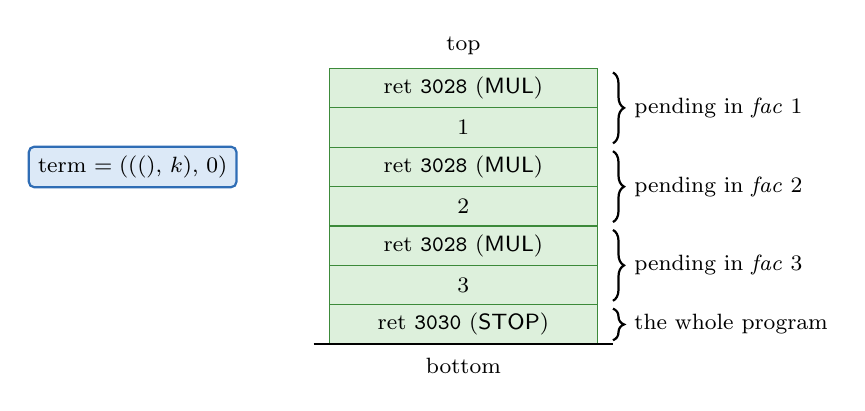
\begin{tikzpicture}
\foreach \v/\c [count=\k from 0] in {{ret \texttt{3030} (\ins{STOP})}/sfill, 3/sfill, {ret \texttt{3028} (\ins{MUL})}/sfill, 2/sfill, {ret \texttt{3028} (\ins{MUL})}/sfill, 1/sfill, {ret \texttt{3028} (\ins{MUL})}/sfill} {
  \node[scell, minimum width=3.4cm] at (0, 0.5*\k) {\v};
}
\draw[thick] (-1.9,-0.25) -- (1.9,-0.25);
\node[font=\footnotesize, anchor=north] at (0,-0.3) {bottom};
\node[font=\footnotesize, anchor=south] at (0,3.3) {top};
\draw[decorate, decoration={brace, amplitude=4pt}, thick] (1.9,1.2) -- node[right=4pt, font=\footnotesize] {pending in \textit{fac} 3} (1.9,0.3);
\draw[decorate, decoration={brace, amplitude=4pt}, thick] (1.9,2.2) -- node[right=4pt, font=\footnotesize] {pending in \textit{fac} 2} (1.9,1.3);
\draw[decorate, decoration={brace, amplitude=4pt}, thick] (1.9,3.2) -- node[right=4pt, font=\footnotesize] {pending in \textit{fac} 1} (1.9,2.3);
\draw[decorate, decoration={brace, amplitude=4pt}, thick] (1.9,0.2) -- node[right=4pt, font=\footnotesize] {the whole program} (1.9,-0.2);
\node[draw=tline, fill=tfill, thick, rounded corners=2pt, font=\footnotesize] at (-4.2,2.0) {term $=\pr{\pr{\unit}{k}}{0}$};
\end{tikzpicture}
\caption{The CAM stack in $\mathit{fac}\ 3$, as the innermost call $f\,0$
starts. Each pending multiplication holds its left operand and a return
address; nothing else survives the call. At the same point, the SECD machine
holds three dump frames of three heap cells each.}
\label{fig:stack}
\end{figure}

% =====================================================================
\section{Where the name comes from}\label{sec:categorical}

So far the CAM has been an engineering design. This section explains its
mathematical origin, without category theory. The idea is to read every piece
of compiled code as a \emph{function}.

\subsection{Code as functions}

By \cref{thm:invariant}, the code $\sem{M}_\rho$ turns an environment in the
term into the value of $M$, and leaves the stack alone. So we can think of it
as a function from environments to values. Let us name a few functions on
values:
\begin{center}
\renewcommand{\arraystretch}{1.2}
\begin{tabular}{@{}l l l@{}}
\toprule
combinator & definition & instructions\\
\midrule
$\cat{Fst}$ & $\cat{Fst}\pr{a}{b} = a$ & \ins{FST}\\
$\cat{Snd}$ & $\cat{Snd}\pr{a}{b} = b$ & \ins{SND}\\
$f\seq g$ & $(f\seq g)(x) = g(f(x))$, first $f$ then $g$ & $f\seq g$\\
$\tpair{f}{g}$ & $\tpair{f}{g}(x) = \pr{f(x)}{g(x)}$ & \ins{PUSH}$\seq f\seq$\ins{SWAP}$\seq g\seq$\ins{CONS}\\
$\Lambda(f)$ & $\Lambda(f)(x) = $ the function $y\mapsto f\pr{x}{y}$ & \ins{CUR} $f$\\
$\cat{App}$ & $\cat{App}\pr{h}{y} = h(y)$ & \ins{APP}\\
$'n$ & $'n(x) = n$, a constant & \ins{QUOTE} $n$\\
\bottomrule
\end{tabular}
\end{center}
With these, the compiler can be written without any instructions:
\[
  \sem{x_i} = \underbrace{\cat{Fst}\seq\cdots\seq\cat{Fst}}_{i}\seq\cat{Snd},
  \qquad
  \sem{\lambda x.M} = \Lambda(\sem{M}),
  \qquad
  \sem{M\,N} = \tpair{\sem{M}}{\sem{N}}\seq\cat{App}.
\]
A variable is a projection out of the environment. A $\lambda$ is a function
that waits for the rest of its environment. An application computes the
function and the argument from the same environment, then applies one to the
other. These are Curien's \emph{categorical combinators}, and the third column
shows that the CAM is simply a machine that executes them: a sequence of
instructions is a composition, read left to right, and
$\tpair{f}{g}$ is implemented by the pairing dance of \cref{fig:dance}. The
original paper even writes \ins{PUSH}, \ins{SWAP} and \ins{CONS} as the
symbols $\langle$, the comma, and $\rangle$ of $\tpair{f}{g}$.

\subsection{The laws}

The combinators obey a handful of equations, which follow directly from
their definitions:
\begin{align*}
\tpair{f}{g}\seq\cat{Fst} &= f &
\tpair{f}{g}\seq\cat{Snd} &= g &
h\seq\tpair{f}{g} &= \tpair{h\seq f}{h\seq g}\\[2pt]
\tpair{h\seq\Lambda(f)}{g}\seq\cat{App} &= \tpair{h}{g}\seq f &
(f\seq g)\seq h &= f\seq(g\seq h) &
\tpair{\cat{Fst}}{\cat{Snd}} &= \mathit{id}
\end{align*}
The first two say that projections undo pairing. The fourth is
$\beta$-reduction in disguise: building a closure of $f$ with environment
$h(x)$ and applying it to $g(x)$ is the same as running $f$ on
$\pr{h(x)}{g(x)}$. That is exactly what \ins{APP} does.

\begin{aside}{What a category theorist would add}
A \emph{category} is any collection of things that compose associatively and
have identities, like our functions. One with pairing and projections obeying
the first three laws is said to have \emph{products}, and one that also has
$\Lambda$ and $\cat{App}$ obeying the fourth law is \emph{cartesian closed}.
A classic result, due to Lambek, is that the simply typed $\lambda$-calculus
and cartesian closed categories describe the same thing~\cite{lambekscott86}:
every $\lambda$-term becomes a combination of these combinators, and every
equation between $\lambda$-terms becomes an equation between combinations.
The CAM takes this correspondence literally and builds a machine whose
instructions are the operations of a cartesian closed category. For this
tutorial, the table and the laws above are all we need. The untyped calculus
we run has no types, but the combinators work the same way.
\end{aside}

\subsection{Why the reading pays off}

Thinking of code as functions has practical consequences. The laws are
program transformations that a compiler may apply. For instance, the law
$\tpair{f}{g}\seq\cat{Fst} = f$ says that the code
\ins{PUSH}$\seq f\seq$\ins{SWAP}$\seq g\seq$\ins{CONS}$\seq$\ins{FST} can be
replaced by $f$, provided $g$ terminates without side effects. The same view
led to a line of research on \emph{explicit substitutions}, calculi in which
environments are part of the term language and which explain all the
classical abstract machines as strategies for applying
substitutions~\cite{acl91}.

% =====================================================================
\section{An implementation on VM16}\label{sec:vm16}

The file \texttt{CAM/cam.asm} implements the machine on VM16, a small
16-bit virtual machine with sixteen registers, a data stack and a return
stack, designed to be implemented in a few hundred lines of assembly on
8-bit processors. One VM16 program, about 3 KB, contains a reader for the
input syntax, the compiler of \cref{sec:compiling}, the CAM interpreter, and a
garbage collector. It runs unchanged on the portable C interpreter and on a
Z80 interpreter.

\subsection{Representation}

The term and the code pointer live in VM16 registers (\texttt{r8} and
\texttt{r9}). The CAM stack is the VM16 data stack, so \ins{PUSH} and \ins{POP}
are single VM16 instructions. Values are 16-bit words:
\begin{itemize}[itemsep=1pt]
\item a number $n$ is stored as $2n+1$, so numbers are odd, need no
  allocation, and range over $-16384$ to $16383$;
\item $\unit$ is 0;
\item pairs and closures are 3-word heap cells: a tag, then the two fields
  (fst and snd, or code address and environment).
\end{itemize}
Tagging makes some arithmetic slightly unusual: $(2a+1)+(2b+1)-1 = 2(a+b)+1$,
so \ins{ADD} is one VM16 addition and one decrement, and comparisons work on
the tagged values directly because tagging preserves the order.
\Cref{fig:memory} shows the memory layout.

\begin{figure}[t]
\centering
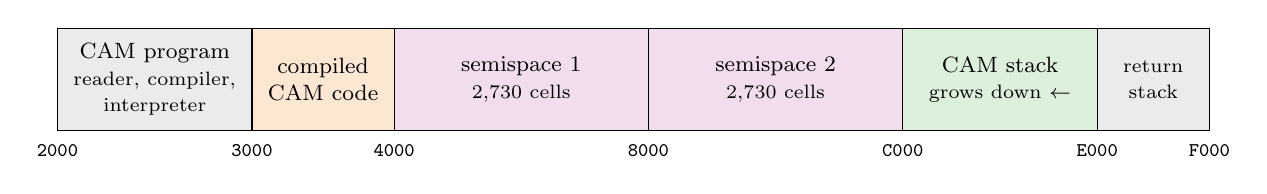
\begin{tikzpicture}[x=0.95cm, y=1cm]
\foreach \a/\b/\l/\c in {0/2.6/{CAM program\\\scriptsize reader, compiler,\\\scriptsize interpreter}/black!8,
                         2.6/4.5/{compiled\\CAM code}/cfill,
                         4.5/7.9/{semispace 1\\\scriptsize 2,730 cells}/hfill,
                         7.9/11.3/{semispace 2\\\scriptsize 2,730 cells}/hfill,
                         11.3/13.9/{CAM stack\\\scriptsize grows down $\leftarrow$}/sfill,
                         13.9/15.4/{\scriptsize return\\\scriptsize stack}/black!8} {
  \draw[fill=\c] (\a,0) rectangle (\b,1.3);
  \node[align=center, font=\footnotesize] at ({(\a+\b)/2},0.65) {\l};
}
\foreach \a/\t in {0/2000, 2.6/3000, 4.5/4000, 7.9/8000, 11.3/C000, 13.9/E000, 15.4/F000}
  \node[font=\scriptsize\ttfamily, anchor=north] at (\a,-0.05) {\t};
\end{tikzpicture}
\caption{Memory layout of \texttt{cam.asm}, not to scale. The compiler writes code from
\texttt{0x3000}. The heap is two 16\,KB semispaces, and the CAM stack grows
down from \texttt{0xE000}.}
\label{fig:memory}
\end{figure}

\subsection{The interpreter}

Each CAM instruction is one opcode byte followed by its operands. The main
loop counts the instruction, fetches the opcode, and jumps through a table:
\begin{lstlisting}
next:   ADDI    r12, 1                  ; count the instruction
        BZ      r12, count_hi
nx_go:  LB      r0, [r9]                ; fetch the opcode
        ADDI    r9, 1
        SHL     r0
        LI      r1, op_table
        ADD     r1, r0
        LW      r1, [r1]
        JR      r1                      ; jump to its handler
\end{lstlisting}
Most handlers are a few instructions long. \ins{PUSH} is \texttt{PUSH r8}
followed by a jump back to \texttt{next}. The longest is \ins{APP}, which
checks that it really has a closure and then builds the new environment:
\begin{lstlisting}
op_app: CALL    reserve                 ; room for one cell
        LW      r1, [r8+2]              ; the closure [C : s]
        ...                             ; (check that r1 is a closure)
app_ok: MOV     r0, r10                 ; term = (s, t)
        ADDI    r10, CELL
        LI      r2, T_PAIR
        SW      r2, [r0]
        LW      r2, [r1+4]
        SW      r2, [r0+2]
        LW      r2, [r8+4]
        SW      r2, [r0+4]
        MOV     r8, r0
        PUSH    r9                      ; the return address
        LW      r9, [r1+2]              ; jump to C
        JMP     next
\end{lstlisting}
The return address is a code address pushed on the CAM stack, exactly as in
the \ins{APP} rule, and \ins{RET} is \texttt{POP r9}.

\subsection{Garbage collection}

The heap is managed by Cheney's copying collector. Allocation is a pointer
increment in the current semispace. When it is full, everything reachable is
copied to the other semispace, and the two swap roles. The collector needs to
know the \emph{roots}, the places outside the heap that may point into it.
In the CAM there are just two: the term and the stack. Two design decisions
keep this simple.

\begin{itemize}[itemsep=2pt]
\item \textbf{Telling pointers apart.} The stack holds heap pointers, numbers
  and return addresses side by side. Numbers are odd, heap cells are at even
  addresses, and return addresses point into the code area, below the heap.
  So the collector can tell them apart by looking at the word alone, and no
  extra tags are needed.
\item \textbf{Collecting only between instructions.} Every instruction that
  allocates first calls \texttt{reserve}, which collects if fewer than two
  cells are free. At that moment, everything live is reachable from the term
  and the stack, and no heap pointer is hidden in a VM16 register.
\end{itemize}

\Cref{fig:heap} shows the heap during the computation of
$\mathit{fib}(20)$, which allocates two cells per call (one in \ins{CONS} and
one in \ins{APP}), 43,784 in all. The heap fills, is collected, and fills
again, 16 times. Hardly anything survives a collection: at most 16 cells,
because the only live data are the environments of the calls in progress.
This is the best case for a copying collector, whose cost depends on what
survives rather than on what was allocated.

\begin{figure}[t]
\centering
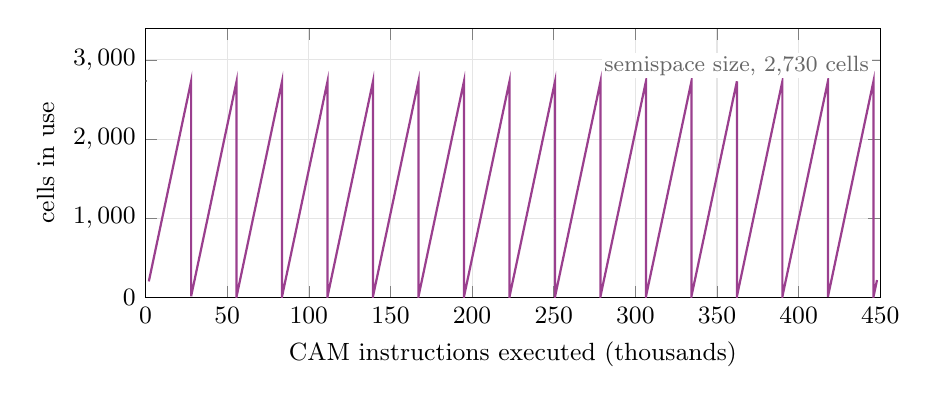
\begin{tikzpicture}
\begin{axis}[width=0.9\textwidth, height=5cm,
  xlabel={CAM instructions executed (thousands)}, ylabel={cells in use},
  xmin=0, xmax=450, ymin=0, ymax=3400, x filter/.code={\pgfmathparse{#1/1000}},
  yticklabel style={/pgf/number format/1000 sep={{,}}},
  grid=major, grid style={black!10},
  every axis plot/.append style={thick}]
\addplot[hline, mark=none] table {
x y
2000 202
4000 396
6000 592
8000 786
10000 982
12000 1176
14000 1372
16000 1566
18000 1762
20000 1956
22000 2152
24000 2348
26000 2542
27912 2729
27912 14
28000 23
30000 217
32000 413
34000 607
36000 803
38000 997
40000 1193
42000 1389
44000 1583
46000 1779
48000 1975
50000 2169
52000 2363
54000 2559
55753 2729
55753 11
56000 35
58000 231
60000 427
62000 621
64000 817
66000 1013
68000 1207
70000 1403
72000 1597
74000 1791
76000 1987
78000 2183
80000 2377
82000 2573
83610 2729
83610 12
84000 50
86000 246
88000 440
90000 636
92000 830
94000 1026
96000 1222
98000 1416
100000 1612
102000 1806
104000 2002
106000 2194
108000 2392
110000 2588
111457 2729
111457 11
112000 64
114000 260
116000 454
118000 650
120000 844
122000 1040
124000 1236
126000 1430
128000 1626
130000 1820
132000 2016
134000 2210
136000 2406
138000 2601
139309 2729
139309 14
140000 81
142000 275
144000 471
146000 667
148000 861
150000 1057
152000 1251
154000 1447
156000 1641
158000 1837
160000 2033
162000 2227
164000 2423
166000 2617
167153 2729
167153 9
168000 93
170000 287
172000 483
174000 679
176000 873
178000 1069
180000 1263
182000 1459
184000 1653
186000 1849
188000 2045
190000 2239
192000 2433
194000 2629
195033 2729
195033 9
196000 103
198000 299
200000 495
202000 689
204000 885
206000 1079
208000 1275
210000 1471
212000 1665
214000 1861
216000 2055
218000 2251
220000 2445
222000 2641
222922 2729
222922 7
224000 115
226000 309
228000 503
230000 699
232000 895
234000 1089
236000 1285
238000 1481
240000 1675
242000 1870
244000 2065
246000 2259
248000 2455
250000 2651
250811 2729
250811 10
252000 126
254000 322
256000 516
258000 712
260000 908
262000 1102
264000 1298
266000 1492
268000 1688
270000 1882
272000 2078
274000 2272
276000 2466
278000 2664
278665 2729
278665 16
280000 147
282000 341
284000 536
286000 731
288000 927
290000 1121
292000 1317
294000 1511
296000 1707
298000 1901
300000 2097
302000 2292
304000 2487
306000 2683
306493 2729
306493 10
308000 158
310000 353
312000 547
314000 744
316000 938
318000 1134
320000 1330
322000 1524
324000 1720
326000 1914
328000 2110
330000 2304
332000 2500
334000 2695
334346 2729
334346 14
336000 175
338000 369
340000 565
342000 759
344000 955
346000 1151
348000 1345
350000 1541
352000 1735
354000 1931
356000 2125
358000 2321
360000 2517
362000 2710
362187 2729
362187 11
364000 189
366000 383
368000 579
370000 773
372000 969
374000 1165
376000 1359
378000 1555
380000 1749
382000 1945
384000 2139
386000 2335
388000 2531
390000 2725
390047 2729
390047 10
392000 202
394000 396
396000 592
398000 786
400000 982
402000 1176
404000 1372
406000 1567
408000 1762
410000 1958
412000 2152
414000 2348
416000 2542
417924 2729
417924 6
418000 15
420000 209
422000 405
424000 601
426000 795
428000 991
430000 1185
432000 1379
434000 1575
436000 1771
438000 1965
440000 2161
442000 2355
444000 2551
445833 2729
445833 7
446000 23
448000 219
};
\addplot[black!50, dashed, domain=0:450] {2730};
\node[font=\footnotesize, anchor=south east, black!60, fill=white, inner sep=1pt] at (axis cs:445,2760) {semispace size, 2,730 cells};
\end{axis}
\end{tikzpicture}
\caption{Heap occupancy while computing $\mathit{fib}(20)$ on the CAM. Each
drop is a garbage collection. The data come from replaying the compiled code
with the implementation's allocation policy, which reproduces its count of 16
collections.}
\label{fig:heap}
\end{figure}

% =====================================================================
\section{Measurements}\label{sec:measure}

How fast is the CAM? The VM16 C interpreter counts the VM16 instructions it
executes, which makes a fair, machine-independent measure.
\Cref{tab:measure} compares the CAM with the SECD machine of the companion
tutorial, implemented on VM16 in the same style, and with
$\mathit{fib}(20)$ written directly in VM16 assembly.

\begin{table}[t]
\centering
\small
\begin{tabular}{@{}l l r r r@{}}
\toprule
program & machine & machine steps & collections & VM16 instructions\\
\midrule
$\mathit{fac}\ 7$, integers & SECD, with $Z$ & 322 transitions & 0 & 29,738\\
 & CAM, with $Z$ & 346 instructions & 0 & 17,528\\
 & CAM, with \textbf{rec} & 171 instructions & 0 & 10,114\\
\midrule
$\mathit{fac}\ 5$, Church numerals & SECD & 52,044 transitions & 49 & 4,086,035\\
 & CAM & 73,681 instructions & 10 & 1,484,236\\
\midrule
$\mathit{fib}(20)$ & SECD, with $Z$ & --- & 702 & 61,161,761\\
 & CAM, with \textbf{rec} & 448,762 instructions & 16 & 6,992,008\\
 & VM16 assembly & --- & --- & 175,169\\
\bottomrule
\end{tabular}
\caption{The same programs on the SECD machine, the CAM, and in hand-written
VM16 code. The VM16 counts include reading and compiling the program, which
is under 0.1\,\% of each run.}
\label{tab:measure}
\end{table}

\begin{figure}[t]
\centering
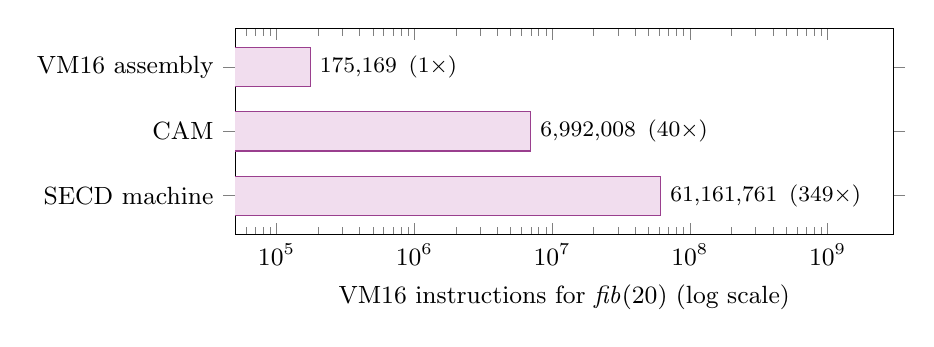
\begin{tikzpicture}
\begin{axis}[xbar, width=0.82\textwidth, height=4.2cm, xmode=log,
  xmin=50000, xmax=3e9, log basis x=10,
  symbolic y coords={VM16 assembly, CAM, SECD machine}, ytick=data,
  y dir=reverse, bar width=0.5cm, enlarge y limits=0.3,
  xlabel={VM16 instructions for $\mathit{fib}(20)$ (log scale)},
  nodes near coords, nodes near coords align={horizontal},
  every node near coord/.append style={font=\footnotesize, anchor=west},
  point meta=explicit symbolic]
\addplot[fill=hfill, draw=hline] coordinates {
  (175169,VM16 assembly) [175,169 \,(1$\times$)]
  (6992008,CAM) [6,992,008 \,(40$\times$)]
  (61161761,SECD machine) [61,161,761 \,(349$\times$)]};
\end{axis}
\end{tikzpicture}
\caption{The cost of $\mathit{fib}(20)$. The CAM is about 9 times faster than
the interpreted SECD machine and about 40 times slower than hand-written
code.}
\label{fig:bars}
\end{figure}

\paragraph{CAM against SECD.} On $\mathit{fib}(20)$ the CAM needs about a
ninth of the work (\cref{fig:bars}). The reasons are the three changes of
\cref{sec:fromsecd}. Variables cost a fixed path of \ins{FST}s instead of a
search by name; a call allocates one pair instead of control-list cells and a
three-cell dump frame; and the SECD implementation also allocates a heap cell
for every number, where the CAM's numbers are tagged words. With fewer
allocations come fewer collections: 16 against 702.

\paragraph{CAM against hand-written code.} The hand-written version keeps $n$
in a register and allocates nothing; each call costs 8 VM16 instructions. The
CAM spends 20.5 instructions per call of $\mathit{fib}$, each costing about
16 VM16 instructions, where they go as follows:
\begin{itemize}[itemsep=2pt]
\item \textbf{Dispatch.} Fetching and dispatching each CAM instruction, plus
  the jump back, takes 10 VM16 instructions, about 4.5 of the 7.0 million.
  A compiler that emitted VM16 code instead of CAM code would remove this.
\item \textbf{Environment traffic.} \ins{PUSH}, \ins{SWAP} and \ins{ACC} make
  up 56\,\% of the CAM instructions executed (\cref{tab:mix}). They exist to
  save and restore environments, which hand-written code keeps in registers.
\item \textbf{Allocation.} Two cells per call, plus the occasional
  collection.
\end{itemize}

\begin{table}[t]
\centering
\small
\begin{tabular}{@{}l r r @{\qquad} l r r@{}}
\toprule
instruction & count & share & instruction & count & share\\
\midrule
\ins{PUSH}  & 98,508 & 22.0\,\% & \ins{BRANCH} & 21,891 & 4.9\,\%\\
\ins{SWAP}  & 76,617 & 17.1\,\% & \ins{RET}    & 21,891 & 4.9\,\%\\
\ins{ACC}   & 76,617 & 17.1\,\% & \ins{LT}     & 21,891 & 4.9\,\%\\
\ins{QUOTE} & 43,782 &  9.8\,\% & \ins{SUB}    & 21,890 & 4.9\,\%\\
\ins{CONS}  & 21,891 &  4.9\,\% & \ins{JUMP}   & 10,946 & 2.4\,\%\\
\ins{APP}   & 21,891 &  4.9\,\% & \ins{ADD}    & 10,945 & 2.4\,\%\\
\bottomrule
\end{tabular}
\caption{The CAM instructions executed for $\mathit{fib}(20)$, 448,762 in all
(plus one \ins{REC} and one \ins{STOP}). Each of the 21,891 calls runs every
instruction of the function body except one branch.}
\label{tab:mix}
\end{table}

On a 4\,MHz Z80, where the VM16 interpreter averages about 250 clock cycles
per VM16 instruction, these figures mean roughly 0.7 seconds for
$\mathit{fac}\ 7$ with \textbf{rec} on the CAM and 2.2 seconds on the SECD
machine, both measured on a Z80 emulator, and an estimated 7 minutes for
$\mathit{fib}(20)$ on the CAM.

% =====================================================================
\section{Variations and descendants}\label{sec:descendants}

\begin{description}[style=nextline, leftmargin=1.2em, itemsep=3pt]
\item[Caml.] The first Caml compiled to the CAM. The machine's main weakness
  showed up there: a curried function of $n$ arguments builds $n-1$
  intermediate closures and environments, as $K\,4\,3$ did in
  \cref{tab:trace2}. Leroy's ZINC machine~\cite{leroy90}, the basis of Caml
  Light and of OCaml's bytecode interpreter, passes several arguments at once
  on a stack and avoids most of them, and it is the subject of an instructive
  report that compares its design with the CAM.
\item[Compiling the CAM further.] Because CAM code is a simple sequence of
  instructions, it can be translated instruction by instruction into native
  code, removing the dispatch overhead measured in \cref{sec:measure}.
\item[Lazy evaluation.] The CAM is call-by-value, but closures can also
  represent suspended computations. Mauny and others studied lazy variants
  in which arguments are passed as closures and evaluated when needed.
\item[Explicit substitutions.] The $\lambda\sigma$-calculus of Abadi, Cardelli,
  Curien and Lévy~\cite{acl91} grew out of the categorical combinators. It
  makes environments part of the calculus and explains the CAM, the SECD
  machine and Krivine's machine~\cite{krivine07} as different strategies for
  carrying out substitutions.
\item[Derivation.] Danvy and colleagues showed that the CAM, like the SECD
  machine, can be derived mechanically from an ordinary evaluator, by
  standard program transformations~\cite{ager03b}. Douence and
  Fradet~\cite{douence98} describe the CAM, the SECD machine and other
  implementations in one framework, as combinations of a few independent
  design choices.
\end{description}

% =====================================================================
\section{Summary}

The CAM evaluates call-by-value $\lambda$-calculus with three registers. It
compiles variables to \emph{positions}, represents environments as
\emph{nested pairs} so that they are ordinary values, and runs
\emph{compiled code} whose return addresses live on the one stack. A
handful of instructions suffices: \ins{ACC}, \ins{QUOTE}, \ins{PUSH},
\ins{SWAP}, \ins{CONS}, \ins{CUR}, \ins{APP} and \ins{RET}, plus a conditional
branch and a recursive closure for practical programming. Read as functions,
those instructions are the combinators of a cartesian closed category, which
is where the machine's name comes from. In practice they make for a machine
that is easy to implement, that needs only the term and the stack as
garbage-collection roots, and that in our measurements is about nine times
faster than the interpreted SECD machine.

% =====================================================================
\section*{Exercises}
\addcontentsline{toc}{section}{Exercises}

\begin{exercise}
Compile $(\lambda f\,x.\,f\,(f\,x))\;(+\;1)\;0$ by hand. How many
instructions does it run? Check your answer with
\texttt{python3 camdis.py} and with the instruction count that
\texttt{cam.v16} prints (45).
\end{exercise}

\begin{exercise}
Translate $\lambda a.\lambda b.\,b\,a$ into categorical combinators, using
the equations for $\sem{x_i}$, $\sem{\lambda x.M}$ and $\sem{M\,N}$. Then use
the laws of \cref{sec:categorical} to show that applying it to two values
$u$ and $v$ gives $v\,u$.
\end{exercise}

\begin{exercise}
Complete the proof of \cref{thm:invariant} for the rules of \textbf{if} and
\textbf{rec}. What goes wrong if \ins{BRANCH} does not pop the environment?
\end{exercise}

\begin{exercise}\label{ex:peephole}
The sequence \ins{PUSH; ACC} $i$\ins{; SWAP} appears whenever a variable is an
operand. Design a single instruction that replaces it, describe its
transition, and estimate from \cref{tab:mix} how many instructions it would
save in $\mathit{fib}(20)$.
\end{exercise}

\begin{exercise}\label{ex:tail}
Every call in the CAM pushes a return address, even a call in tail position
such as $f\,(n-1)\,(a+n)$ in an accumulating loop. Design a tail-call
instruction (compare \ins{TAP} in the compiled SECD machine), show which
sequence the compiler should replace with it, and explain why the stack then
stays bounded for \verb|(rec f.\n a.if (= n 0) a (f (- n 1) (+ a n))) 3000 0|.
\end{exercise}

\begin{exercise}
Variable access costs $i+1$ steps for index $i$. Describe an alternative
representation where every variable costs one step, such as copying the
values a closure needs into a flat vector when it is created. What does
closure creation cost then? Which choice did Leroy make in ZINC?
\end{exercise}

\begin{exercise}
In \texttt{cam.asm}, \texttt{=} and \texttt{<} return 1 or 0, and \textbf{if}
only accepts numbers. Change them to work with Church booleans
$\lambda x\,y.x$ and $\lambda x\,y.y$. How can \ins{BRANCH} recognise them?
\end{exercise}

\begin{exercise}
Add pairs to the source language: $\langle M, N\rangle$, $\mathit{fst}\,M$
and $\mathit{snd}\,M$. Show that they compile to instructions the CAM already
has, and that the categorical law $\tpair{f}{g}\seq\cat{Fst} = f$ then
justifies an optimisation.
\end{exercise}

\begin{exercise}
In \cref{fig:heap}, at most 16 cells survive a collection. Explain where this
bound comes from, in terms of the depth of the recursion and the cells that a
pending call of $\mathit{fib}$ keeps alive.
\end{exercise}

\begin{exercise}
Write a CAM interpreter in a language of your choice from the reference card
alone, and test it on the examples of \cref{sec:examples,sec:recursion}.
\end{exercise}

% =====================================================================
\section{Reference card}\label{sec:card}

\begin{center}
\small
\renewcommand{\arraystretch}{1.15}
\begin{tabular}{@{}l r@{\;}c@{\;}l@{}}
\toprule
\multicolumn{4}{@{}l}{\textbf{Machine} \quad (start $\cs{\unit}{P}{\varepsilon}$; halt at \ins{STOP}, with the result in the term)}\\
\midrule
\ins{ACC} $i$ & $\cs{t}{\ins{ACC}\,i\seq C}{S}$ &$\to$& $\cs{\mathit{snd}(\mathit{fst}^i(t))}{C}{S}$\\
\ins{QUOTE} $n$ & $\cs{t}{\ins{QUOTE}\,n\seq C}{S}$ &$\to$& $\cs{n}{C}{S}$\\
\ins{PUSH} & $\cs{t}{\ins{PUSH}\seq C}{S}$ &$\to$& $\cs{t}{C}{t.S}$\\
\ins{SWAP} & $\cs{t}{\ins{SWAP}\seq C}{s.S}$ &$\to$& $\cs{s}{C}{t.S}$\\
\ins{CONS} & $\cs{t}{\ins{CONS}\seq C}{s.S}$ &$\to$& $\cs{\pr{s}{t}}{C}{S}$\\
\ins{CUR} $C'$ & $\cs{t}{\ins{CUR}\,C'\seq C}{S}$ &$\to$& $\cs{\clo{C'}{t}}{C}{S}$\\
\ins{APP} & $\cs{\pr{\clo{C'}{s}}{t}}{\ins{APP}\seq C}{S}$ &$\to$& $\cs{\pr{s}{t}}{C'}{C.S}$\\
\ins{RET} & $\cs{t}{\ins{RET}\seq C}{C'.S}$ &$\to$& $\cs{t}{C'}{S}$\\
\textit{op} & $\cs{n_2}{\textit{op}\seq C}{n_1.S}$ &$\to$& $\cs{n_1\mathbin{\textit{op}}n_2}{C}{S}$\\
\ins{BRANCH} & $\cs{b}{\ins{BRANCH}\,C_1\,C_2\seq C}{s.S}$ &$\to$& $\cs{s}{C_b\seq C}{S}$\\
\ins{REC} $C'$ & $\cs{t}{\ins{REC}\,C'\seq C}{S}$ &$\to$& $\cs{k}{C}{S}$, \ $k = \clo{C'}{\pr{t}{k}}$\\
\midrule
\multicolumn{4}{@{}l}{\textbf{Compiler} \quad ($\rho$ = names in scope, innermost first)}\\
\midrule
variable & $\sem{x}_\rho$ &$=$& \ins{ACC} (position of $x$ in $\rho$)\\
constant & $\sem{n}_\rho$ &$=$& \ins{QUOTE} $n$\\
abstraction & $\sem{\lambda x.M}_\rho$ &$=$& \ins{CUR} $(\sem{M}_{x:\rho}\seq\ins{RET})$\\
application & $\sem{M\,N}_\rho$ &$=$& \ins{PUSH}$\seq\sem{M}_\rho\seq$\ins{SWAP}$\seq\sem{N}_\rho\seq$\ins{CONS}$\seq$\ins{APP}\\
operator & $\sem{\textit{op}\,M\,N}_\rho$ &$=$& \ins{PUSH}$\seq\sem{M}_\rho\seq$\ins{SWAP}$\seq\sem{N}_\rho\seq\textit{op}$\\
conditional & $\sem{\textbf{if}\,c\,t\,e}_\rho$ &$=$& \ins{PUSH}$\seq\sem{c}_\rho\seq$\ins{BRANCH} $\sem{t}_\rho\ \sem{e}_\rho$\\
recursion & $\sem{\textbf{rec}\,f.\lambda x.M}_\rho$ &$=$& \ins{REC} $(\sem{M}_{x:f:\rho}\seq\ins{RET})$\\
\midrule
\multicolumn{4}{@{}l}{\textbf{Combinators}}\\
\midrule
\multicolumn{4}{@{}l}{$\sem{x_i} = \cat{Fst}^i\seq\cat{Snd}$ \qquad $\sem{\lambda x.M} = \Lambda(\sem{M})$ \qquad $\sem{M\,N} = \tpair{\sem{M}}{\sem{N}}\seq\cat{App}$}\\
\multicolumn{4}{@{}l}{$\tpair{f}{g}\seq\cat{Fst} = f$ \quad $\tpair{f}{g}\seq\cat{Snd} = g$ \quad $\tpair{h\seq\Lambda(f)}{g}\seq\cat{App} = \tpair{h}{g}\seq f$}\\
\bottomrule
\end{tabular}
\end{center}

% =====================================================================
\begin{thebibliography}{99}
\small

\bibitem{acl91}
M.~Abadi, L.~Cardelli, P.-L. Curien, and J.-J. Lévy.
\newblock Explicit substitutions.
\newblock \emph{Journal of Functional Programming}, 1(4):375--416, 1991.

\bibitem{ager03b}
M.~S. Ager, D.~Biernacki, O.~Danvy, and J.~Midtgaard.
\newblock From interpreter to compiler and virtual machine: a functional
  derivation.
\newblock Technical Report RS-03-14, BRICS, University of Aarhus, 2003.

\bibitem{cam85}
G.~Cousineau, P.-L. Curien, and M.~Mauny.
\newblock The categorical abstract machine.
\newblock In \emph{Functional Programming Languages and Computer Architecture
  (FPCA)}, volume 201 of \emph{LNCS}, pages 50--64. Springer, 1985.

\bibitem{cam87}
G.~Cousineau, P.-L. Curien, and M.~Mauny.
\newblock The categorical abstract machine.
\newblock \emph{Science of Computer Programming}, 8(2):173--202, 1987.

\bibitem{curien86}
P.-L. Curien.
\newblock \emph{Categorical Combinators, Sequential Algorithms and Functional
  Programming}.
\newblock Pitman, 1986. Second edition, Birkhäuser, 1993.

\bibitem{debruijn72}
N.~G. de~Bruijn.
\newblock Lambda calculus notation with nameless dummies, a tool for automatic
  formula manipulation, with application to the {C}hurch--{R}osser theorem.
\newblock \emph{Indagationes Mathematicae}, 34:381--392, 1972.

\bibitem{douence98}
R.~Douence and P.~Fradet.
\newblock A systematic study of functional language implementations.
\newblock \emph{ACM Transactions on Programming Languages and Systems},
  20(2):344--387, 1998.

\bibitem{henderson80}
P.~Henderson.
\newblock \emph{Functional Programming: Application and Implementation}.
\newblock Prentice-Hall, 1980.

\bibitem{krivine07}
J.-L. Krivine.
\newblock A call-by-name lambda-calculus machine.
\newblock \emph{Higher-Order and Symbolic Computation}, 20(3):199--207, 2007.

\bibitem{lambekscott86}
J.~Lambek and P.~J. Scott.
\newblock \emph{Introduction to Higher Order Categorical Logic}.
\newblock Cambridge University Press, 1986.

\bibitem{landin64}
P.~J. Landin.
\newblock The mechanical evaluation of expressions.
\newblock \emph{The Computer Journal}, 6(4):308--320, 1964.

\bibitem{leroy90}
X.~Leroy.
\newblock The {ZINC} experiment: an economical implementation of the {ML}
  language.
\newblock Technical Report 117, INRIA, 1990.

\end{thebibliography}

\end{document}
